\documentclass[12pt,letterpaper]{article}\usepackage[]{graphicx}\usepackage[]{color}
%% maxwidth is the original width if it is less than linewidth
%% otherwise use linewidth (to make sure the graphics do not exceed the margin)
\makeatletter
\def\maxwidth{ %
  \ifdim\Gin@nat@width>\linewidth
    \linewidth
  \else
    \Gin@nat@width
  \fi
}
\makeatother

\definecolor{fgcolor}{rgb}{0.345, 0.345, 0.345}
\newcommand{\hlnum}[1]{\textcolor[rgb]{0.686,0.059,0.569}{#1}}%
\newcommand{\hlstr}[1]{\textcolor[rgb]{0.192,0.494,0.8}{#1}}%
\newcommand{\hlcom}[1]{\textcolor[rgb]{0.678,0.584,0.686}{\textit{#1}}}%
\newcommand{\hlopt}[1]{\textcolor[rgb]{0,0,0}{#1}}%
\newcommand{\hlstd}[1]{\textcolor[rgb]{0.345,0.345,0.345}{#1}}%
\newcommand{\hlkwa}[1]{\textcolor[rgb]{0.161,0.373,0.58}{\textbf{#1}}}%
\newcommand{\hlkwb}[1]{\textcolor[rgb]{0.69,0.353,0.396}{#1}}%
\newcommand{\hlkwc}[1]{\textcolor[rgb]{0.333,0.667,0.333}{#1}}%
\newcommand{\hlkwd}[1]{\textcolor[rgb]{0.737,0.353,0.396}{\textbf{#1}}}%

\usepackage{framed}
\makeatletter
\newenvironment{kframe}{%
 \def\at@end@of@kframe{}%
 \ifinner\ifhmode%
  \def\at@end@of@kframe{\end{minipage}}%
  \begin{minipage}{\columnwidth}%
 \fi\fi%
 \def\FrameCommand##1{\hskip\@totalleftmargin \hskip-\fboxsep
 \colorbox{shadecolor}{##1}\hskip-\fboxsep
     % There is no \\@totalrightmargin, so:
     \hskip-\linewidth \hskip-\@totalleftmargin \hskip\columnwidth}%
 \MakeFramed {\advance\hsize-\width
   \@totalleftmargin\z@ \linewidth\hsize
   \@setminipage}}%
 {\par\unskip\endMakeFramed%
 \at@end@of@kframe}
\makeatother

\definecolor{shadecolor}{rgb}{.97, .97, .97}
\definecolor{messagecolor}{rgb}{0, 0, 0}
\definecolor{warningcolor}{rgb}{1, 0, 1}
\definecolor{errorcolor}{rgb}{1, 0, 0}
\newenvironment{knitrout}{}{} % an empty environment to be redefined in TeX

\usepackage{alltt}
 \usepackage[left=2cm,right=2cm,top=2cm,bottom=2cm]{geometry}
\usepackage[ansinew]{inputenc}
\usepackage[spanish]{babel}
\usepackage{amsmath}
\usepackage{amsfonts}
\usepackage{amssymb}
\usepackage{dsfont}
\usepackage{multicol} 
\usepackage{subfigure}
\usepackage{graphicx}
\usepackage{float} 
\usepackage{verbatim} 
\usepackage[left=2cm,right=2cm,top=2cm,bottom=2cm]{geometry}
\usepackage{fancyhdr}
\pagestyle{fancy} 
\fancyhead[LO]{\leftmark}
\usepackage{caption}
\newtheorem{definicion}{Definci\'on}
\IfFileExists{upquote.sty}{\usepackage{upquote}}{}
\begin{document}

\begin{titlepage}
\setlength{\unitlength}{1 cm} %Especificar unidad de trabajo


\begin{center}
\textbf{{\large UNIVERSIDAD DE EL SALVADOR}\\
{\large FACULTAD MULTIDISCIPLINARIA DE OCCIDENTE}\\
{\large DEPARTAMENTO DE MATEM\'ATICA}}\\[0.50 cm]

\begin{picture}(18,4)
 \put(7,0){
\includegraphics[width=4cm]{minerva.jpg}}
\end{picture}
\\[0.25 cm]

\textbf{{\large Licenciatura en Estad\'istica}\\[1.25cm]
{\large Control Estadistico del Paquete R }\\[2 cm]
%\setlength{\unitlength}{1 cm}
{\large  \textbf{''UNIDAD SEIS"}}\\[3 cm]
{\large Alumna:}\\
{\large Erika Beatr\'i Guillen\'en Pineda}\\[2cm]
{\large Fecha de elaboraci\'on}\\
Santa Ana - \today }
\end{center}
\end{titlepage}

\newtheorem{teorema}{Teorema}
\newtheorem{prop}{Proposici\'on}[section]


\lhead{PR\'ACTICA 24}
\lfoot{LICENCIATURA EN ESTAD\'ISTICA}
\cfoot{UESOCC}
\rfoot{\thepage}
%\pagestyle{fancy} 

\setcounter{page}{1}
\newpage
\section{INTRODUCCI\'ON}
En muchos casos pr\'acticos existe la necesidad de realizar o de hacer comparaciones entre la media de una caracter\'istica en diferentes niveles o grupos bajo un nivel de significancia $alfa$ prefijado; en estos casos el \textbf{AN\'ALISIS DE VARIANZA} es la t\'ecnica estad\'istica m\'as adecuada para poder llevar a cabo simult\'aneamente dichas comparaciones. El An\'alisisde Varianza, descompone la variabilidad total (VT) de la variable de inter\'es en dos fuentes de variabilidad mutuamente independientes: una debida a los efectos de los grupos o variabilidad explicada por los grupos (VE) y otra debida a los errores (perturbaciones) o variabilidad no explicada (VNE). Es com\'un, en los Dise\~nos de Experimentos llamar a cada uno de esos niveles o grupos con el nombre de "tratamientos". Esta t\'ecnica tiene como objetivo identificar la importancia de los diferentes grupos en el estudio y determinar la influencia de ellos sobre la variable de inter\'es.\\

Si nuestra variable de inter\'es,la cual representaremos por  y, es continua una manera muy conveniente de representar las observaciones es por medio de la siguiente ecuaci\'on:

\begin{center}
\textbf{$y_\ij$ = $\µ_i$ + $u_\ij$}
\end{center}

Donde: 

\begin{itemize}
  \item $y_\ij$: Representa la j-\'esima observaci\'on correspondiente al i-\'esimo grupo.
  \item $\µ_i$: Representa la media del i-\'esimo grupo (o tratamiento)
  \item $u_\ij$: Representa un componente de error aleatorio, llamado perturbaciones, que incorpora todas las dem\'as fuentes de variabilidad del experimento (no incluidas en los grupos o tratamientos).
\end{itemize}

A la ecuaci\'on anterior, se le conoce con el nombre de "modelos en medias". Una forma alternativa y mucho m\'as interesante de escribirlo es considerando el caso en que $t_i$ = $\µ_i$ - $\µ$, por lo que el modelo se convierte en: $y_\ij$ = $\µ$ + $t_i$ + $e_\ij$\\

El cual recibe el nombre de "modelos de efectos"; pues el t\'ermino $t_i$ representa el efecto del grupo i-\'esimo (o tratamiento i-\'esimo). Y debe cumplirse que la sumatoria de $t_i$=0.\\
 
Las perturbaciones como ya se mencion\'o representan la variabilidad intr\'inseca del experimento y supondremos que verifican las hip\'otesis siguientes (en caso de duda hay que contrastarlas):\\[1.00 cm]

\textbf{Hip\'otesis:}
\begin{itemize}

  \item El promedio de las perturbaciones escero, es decir, se cumple que:\\
  E[$u_\ij$] = 0; para todo i,j.
  
  \item La varianza de las perturbaciones es constante, es decir, se cumple que:\\
  var($u_\ij$) = $sigma^2$; para todo $i,j$.
 
  \item La distribuci\'on de las perturbaciones debe ser normal, es decir se cumple que:\\ $u_\ij$ = N(0; $sigma^2$) =; para todo $i,j$.
  
  \item Las perturbaciones son independientes, es decir se cumple que:\\
  cov($u_\ij$; $u_\ i^'\ j^'$)=0; para todo $i$ distinto de $i^'$, y para todo $j$ distinto de $j^'$
\end{itemize}

Las cuatro hip\'otesis anteriores sobre las perturbaciones que son las hip\'otesis b\'asicas del modelo, pueden resumirse en (IID significa que son variables aleatorias independientes e id\'enticamente distribuidas):\\

$u_\ij$ = $NIID$ N(0; $sigma^2$) =; para todo i,j.\\

Si por ejemplo tenemos una \'unica caracter\'istica de inter\'es y existen k grupos (o tratamientos) en los cuales se mide \'esta, podr\'ia estarse interesado en probar la igualdad de las media en cada una de los grupos (tratamientos).\\

La hip\'otesis a probar son:\\
$H_o$: $\µ_1$ = $\µ_2$ = $\µ_3$ ... $\µ_k$\\
$H_1$: $\µ_i$ distinto $\µ_j$; para al menos un par $i$ distinto de $j$\\

Las cuales en t\'erminos de los efectos de grupos, son equivalente a las siguientes hip\'otesis:\\ 
$H_o$: $t_1$ = $t_2$ ... $t_k$ = 0\\
$H_1$: $t_i$ distinto 0; para al menos un $i$\\

En el caso m\'as general, como nunca podemos estudiara toda la poblaci\'on, sino lo que tenemos es una muestra aleatoria de ella (en realidad es una muestra aleatoria de cada grupo); suceder\'a que: 

\begin{itemize}
  \item k es el n\'umero de grupos de inter\'es (tratamientos).
  \item $n_i$ es el n\'umero de observaciones pertenecientes al grupo $i$
  \item N = a la sumatoria de $n_i$ n\'umero total de observaciones.
\end{itemize}

Con dicha muestra debemos contrastarlas hip\'otesis anteriores y estimar cada uno de los par\'ametros del modelo. No resulta dif\'icil verificar utilizando el m\'etodo de m\'axima verosimilitud que el modelo estimado para los datos es:\\

$\^y_\ij$ = $\^\µ$ + $\^t_i$ + $\^u_\ij$\\

Donde: 
\begin{itemize}
  \item $\^\µ$ = $\~y_..$
  \item $\^t_i$ = $\~y_i.$ - $\~y_..$
  \item $\^u_\ij$ = $y_\ij$ - $\~y_i.$
\end{itemize}

Y se tendr\'an las siguientes medidas de inter\'es: 
\begin{itemize}
  \item $\~y_i.$ es el promedio de la caracter\'istica de inter\'es en el grupo $i$. 
 \item $\~y_..$ es la media general de la caracter\'istica de inter\'es.  
\end{itemize}

El An\'alisis de Varianza establece que se debe cumplir la siguiente relaci\'on (al ser cada uno de las fuentes ortogonales entre s\'i):\\

$VT$ = $VE$ + $VNE$\\

Donde: 
\begin{itemize}
  \item VT es la variabilidad total del experimento.
  \item VE es la variabilidad explicada por los grupos o tratamientos.
  \item VNE es la variabilidad no explicada o residual. 
\end{itemize}

Para poder contrastar simult\'aneamente la igualdad de las k medias, se hace uso de lo siguiente:\\

Grupos o Tratamientos:
\begin{itemize}
  \item Sumas de Cuadrados: VE.
  \item Grados de Libertad: $K-1$
  \item Medias de Cuadrados: $MCE$ = $VE$ / $K-1$ 
  \item $F_o$: $F_o$ = $MCE$/$MCNE$
\end{itemize}

Error o perturbaciones:
\begin{itemize}
  \item Sumas de Cuadrados: $VNE$.
  \item Grados de Libertad: $N - K$
  \item Medias de Cuadrados: $MCNE$ = $VNE$ / $N-1$ 
\end{itemize}

Total:
\begin{itemize}
  \item Sumas de Cuadrados: $VT$ = $VE$ + $VNE$
  \item rados de Libertad: $N - 1$
\end{itemize}

De tal modo que la hip\'otesis nula se rechaza (a un nivel de confianza del  100(1 - $alfa$)\%) si\\

$F_o$$>$$F_\ alfa,(K-1),(N-K)$


\section{Ejemplo 1:}

El Ministerio de Educaci\'on est\'a interesado en implementar tres programas de estudio; con el objetivo de medir la habilidad de lectura en los alumnos. Para ello, se eligen alumnos del sexto grado de un Colegio de San Salvador, 27 alumnos fueron asignados al azar, a cada uno de los tres grupos. Se utiliz\'o un programa diferente en cada grupo, se llev\'o a cabo un examen al inicio y al final de la implementaci\'on de los programas, los valores obtenidos representan la diferencia que hay entre la nota del examen que se hizo al inicio y al finalde la implementaci\'on del programa. Los datos se muestran en el siguiente cuadro:
\begin{knitrout}
\definecolor{shadecolor}{rgb}{0.969, 0.969, 0.969}\color{fgcolor}\begin{kframe}
\begin{alltt}
\hlstd{programa} \hlkwb{<-} \hlkwd{c}\hlstd{(}\hlnum{1}\hlstd{,} \hlnum{2}\hlstd{,} \hlnum{3}\hlstd{)}
\hlstd{programa}
\end{alltt}
\begin{verbatim}
## [1] 1 2 3
\end{verbatim}
\begin{alltt}
\hlstd{Observaciones_1} \hlkwb{<-} \hlkwd{c}\hlstd{(}\hlnum{20}\hlstd{,} \hlnum{18}\hlstd{,} \hlnum{18}\hlstd{,} \hlnum{23}\hlstd{,} \hlnum{22}\hlstd{,} \hlnum{17}\hlstd{,} \hlnum{15}\hlstd{,} \hlnum{13}\hlstd{,} \hlnum{21}\hlstd{)}
\hlstd{Observaciones_1}
\end{alltt}
\begin{verbatim}
## [1] 20 18 18 23 22 17 15 13 21
\end{verbatim}
\begin{alltt}
\hlstd{Observaciones_2} \hlkwb{<-} \hlkwd{c}\hlstd{(}\hlnum{15}\hlstd{,} \hlnum{20}\hlstd{,} \hlnum{13}\hlstd{,} \hlnum{12}\hlstd{,} \hlnum{16}\hlstd{,} \hlnum{17}\hlstd{,} \hlnum{21}\hlstd{,} \hlnum{15}\hlstd{,} \hlnum{13}\hlstd{)}
\hlstd{Observaciones_2}
\end{alltt}
\begin{verbatim}
## [1] 15 20 13 12 16 17 21 15 13
\end{verbatim}
\begin{alltt}
\hlstd{Observaciones_3} \hlkwb{<-} \hlkwd{c}\hlstd{(}\hlnum{12}\hlstd{,} \hlnum{15}\hlstd{,} \hlnum{18}\hlstd{,} \hlnum{20}\hlstd{,} \hlnum{18}\hlstd{,} \hlnum{17}\hlstd{,} \hlnum{10}\hlstd{,} \hlnum{24}\hlstd{,} \hlnum{16}\hlstd{)}
\hlstd{Observaciones_3}
\end{alltt}
\begin{verbatim}
## [1] 12 15 18 20 18 17 10 24 16
\end{verbatim}
\end{kframe}
\end{knitrout}

Contraste a un nivel de significancia del 5\% de que los tres m\'etodos de lectura producen el mismo efecto en la habilidad de lectura de los alumnos.

\begin{itemize}
  \item La variable en estudio es la habilidad de lectura.
  \item El modelo que genera los datos es el siguiente:\\
  $\^y_\ij$ = $\^\µ$ + $\^t_i$ + $\^u_\ij$
  \item Las hip\'otesis son las siguientes:\\
  $H_o$: $\µ_1$ = $\µ_2$ = $\µ_3$\\
  $H_1$: $\µ_1$ distinto $\µ_2$ distinto $\µ_3$
  \item Ejecutar el script "anova1.R"

\begin{knitrout}
\definecolor{shadecolor}{rgb}{0.969, 0.969, 0.969}\color{fgcolor}\begin{kframe}
\begin{alltt}
\hlcom{# Se digitan las observaciones }

\hlstd{notas} \hlkwb{<-} \hlkwd{c}\hlstd{(}\hlnum{20}\hlstd{,} \hlnum{18}\hlstd{,} \hlnum{18}\hlstd{,} \hlnum{23}\hlstd{,} \hlnum{22}\hlstd{,} \hlnum{17}\hlstd{,} \hlnum{15}\hlstd{,} \hlnum{13}\hlstd{,} \hlnum{21}\hlstd{,} \hlnum{15}\hlstd{,} \hlnum{20}\hlstd{,} \hlnum{13}\hlstd{,} \hlnum{12}\hlstd{,} \hlnum{16}\hlstd{,} \hlnum{17}\hlstd{,} \hlnum{21}\hlstd{,}
           \hlnum{15}\hlstd{,} \hlnum{13}\hlstd{,} \hlnum{12}\hlstd{,} \hlnum{15}\hlstd{,} \hlnum{18}\hlstd{,} \hlnum{20}\hlstd{,} \hlnum{18}\hlstd{,} \hlnum{17}\hlstd{,} \hlnum{10}\hlstd{,} \hlnum{24}\hlstd{,} \hlnum{16}\hlstd{)}

\hlcom{# Se crea un vector de datos en el cual se diferencia cada uno de los }
\hlcom{# programas  de estudio los primeros 9 corresponden al primer programa }
\hlcom{# de estudio, etiquetado por P1; los siguientes 9 corresponden al segundo }
\hlcom{# programa, P2, y lo mismo para el tercero. }

\hlstd{programas} \hlkwb{<-} \hlkwd{gl}\hlstd{(}\hlkwc{n}\hlstd{=}\hlnum{3}\hlstd{,} \hlkwc{k}\hlstd{=}\hlnum{9}\hlstd{,} \hlkwc{labels}\hlstd{=}\hlkwd{c}\hlstd{(}\hlstr{"P1"}\hlstd{,} \hlstr{"P2"}\hlstd{,} \hlstr{"P3"}\hlstd{))}

\hlcom{#gl genera factores especificados por un patr\textbackslash{}'on en sus niveles }
\hlcom{# n especifica que se crea una variable factor con tres niveles diferentes }
\hlcom{# etiquetados por "P1", "P2" y "P3". La instrucci\textbackslash{}'on k=9 indica que a los }
\hlcom{# primeros 9 elementos se les asignar\textbackslash{}'a el valor de P1; a los siguientes 9 }
\hlcom{# el valor de P2; y a los \textbackslash{}'ultimos 9 el valor de P3. }

\hlcom{#Crea la matriz de datos que contendrá la informaci\textbackslash{}'on del experimento (es }
\hlcom{# necesario que los datos est\textbackslash{}'en organizados en una hoja de datos).}

\hlstd{datos} \hlkwb{<-} \hlkwd{data.frame}\hlstd{(}\hlkwc{notas} \hlstd{= notas,} \hlkwc{programas} \hlstd{= programas);datos}
\end{alltt}
\begin{verbatim}
##    notas programas
## 1     20        P1
## 2     18        P1
## 3     18        P1
## 4     23        P1
## 5     22        P1
## 6     17        P1
## 7     15        P1
## 8     13        P1
## 9     21        P1
## 10    15        P2
## 11    20        P2
## 12    13        P2
## 13    12        P2
## 14    16        P2
## 15    17        P2
## 16    21        P2
## 17    15        P2
## 18    13        P2
## 19    12        P3
## 20    15        P3
## 21    18        P3
## 22    20        P3
## 23    18        P3
## 24    17        P3
## 25    10        P3
## 26    24        P3
## 27    16        P3
\end{verbatim}
\begin{alltt}
\hlcom{#Aplicando el an\textbackslash{}'alisis de varianza}

\hlstd{mod1} \hlkwb{<-} \hlkwd{aov}\hlstd{(notas} \hlopt{~} \hlstd{programas,} \hlkwc{data} \hlstd{= datos)}

\hlcom{# la expresi\textbackslash{}'on notas ~ programas indica que se trata de explicar la }
\hlcom{# variabilidad de la variable "notas" mediante el conocimiento (o en }
\hlcom{# funci\textbackslash{}'on de los valores) de la variable "programas", es decir, el }
\hlcom{# nombre del factor que distingue a qu\textbackslash{}'e grupo pertenece cada observaci\textbackslash{}'on. }
\hlcom{# Finalmente en "data = datos" se especifica el nombre de la hoja de datos.}

\hlcom{# Mostrando la tabla ANOVA }

\hlkwd{summary}\hlstd{(mod1)}
\end{alltt}
\begin{verbatim}
##             Df Sum Sq Mean Sq F value Pr(>F)
## programas    2  36.22   18.11    1.44  0.257
## Residuals   24 301.78   12.57
\end{verbatim}
\begin{alltt}
\hlcom{# Para hacer un diagn\textbackslash{}'ostico de las perturbaciones del modelo }

\hlkwd{plot}\hlstd{(mod1)}
\end{alltt}
\end{kframe}
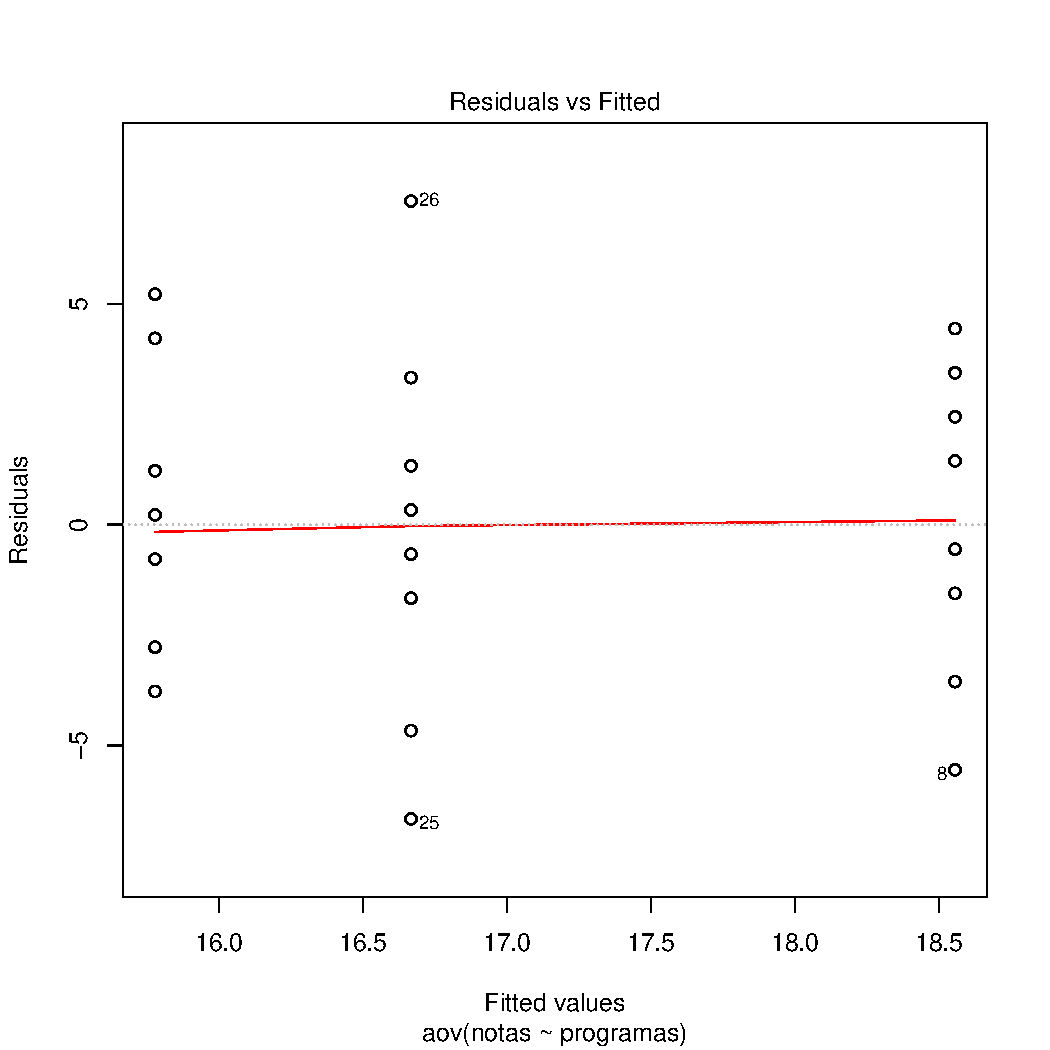
\includegraphics[width=\maxwidth]{figure/unnamed-chunk-2-1} 

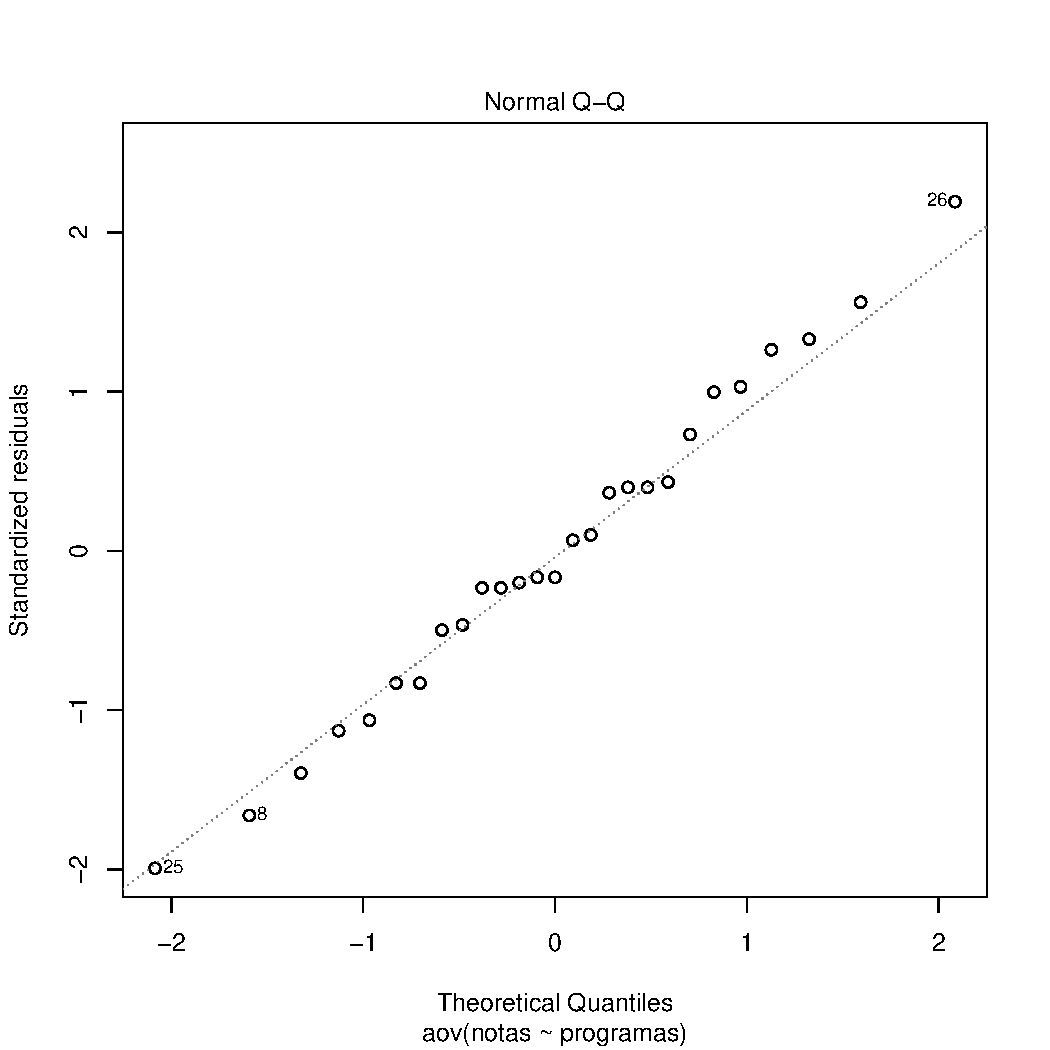
\includegraphics[width=\maxwidth]{figure/unnamed-chunk-2-2} 

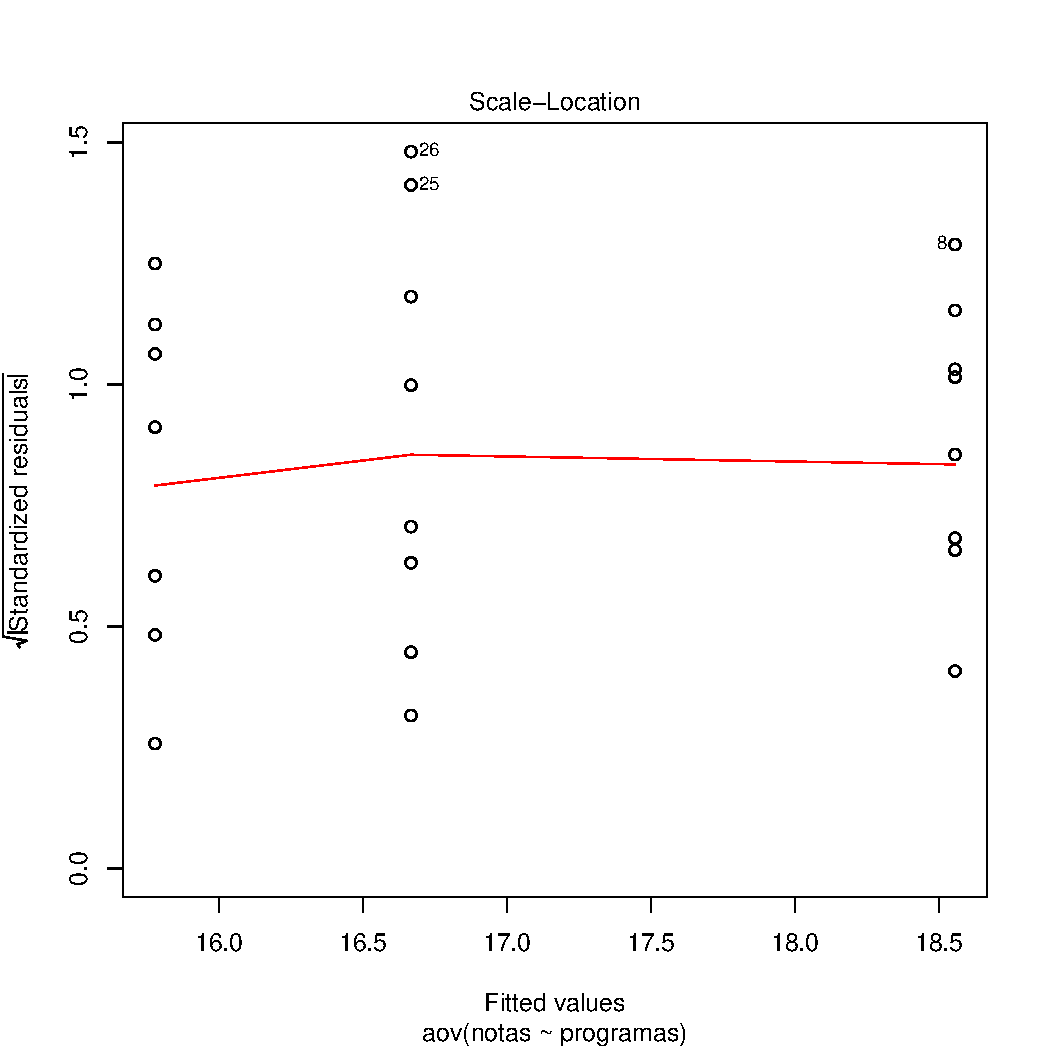
\includegraphics[width=\maxwidth]{figure/unnamed-chunk-2-3} 

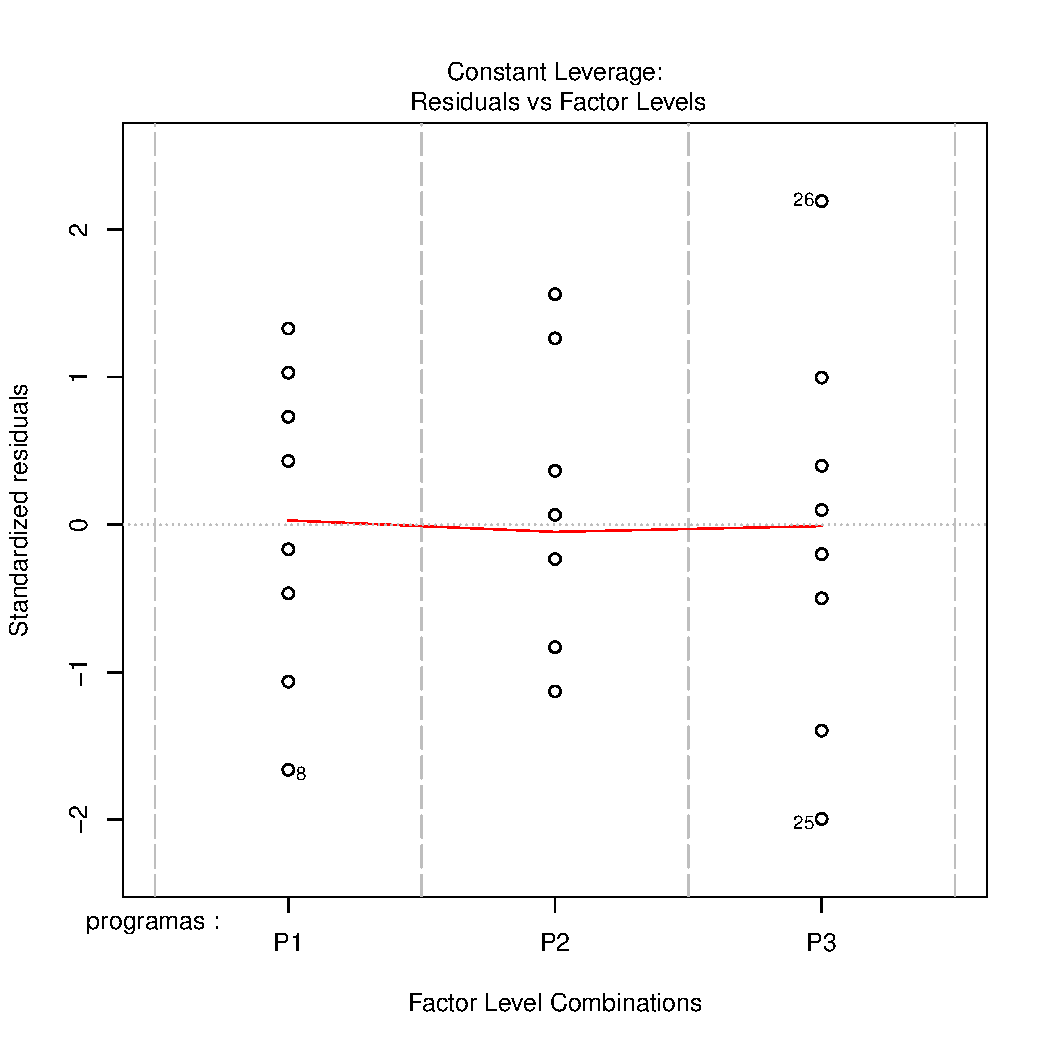
\includegraphics[width=\maxwidth]{figure/unnamed-chunk-2-4} 

\end{knitrout}



En la mayor\'ia de los casos los datos a analizar se encontrar\'an en un archivo ya existente, para esto lo recomendable es que en el archivo tenga la estructura siguiente: una columna en la cual contenga las observaciones de la muestra de nuestra variable dependiente, y una columna adicional con el cual se identifique el grupo de pertenencia de cada una de las observaciones, siendo lo recomendable que sea una variable de tipo car\'acter; si este fuere el caso \'unicamente debemos convertir a la variable de tipo car\'acter en una variable de tipo y factor y realizar el procedimiento descrito en el ejemplo anterior.\\

En algunos casos, aunque sea muy raro, el archivo contendr\'a la siguiente estructura: contendr\'a tantas columnas como grupos se est\'en considerando, y encada columna se contar\'an con las observaciones correspondientes a dicho grupos, el n\'umero de observaciones no tiene porque ser los mismos por lo que se leer\'an unos cuantos datos faltantes. Veamos el siguiente ejemplo.\\


\section{COMENTARIOS FINALES DEL ANOVA.}

El ANOVA en su versi\'on param\'etrica del test de la $F$, como todos los procedimientos estad\'isticos, tiene un cierto grado de robustez frente a un relativo incumplimiento de alguna(s) de sus hip\'otesis. En concreto, el test de la $F$ soporta mejor las deficiencias respecto a la normalidad que las relacionadas con la homocedasticidad. En todo caso, los test son menos sensibles a las desviaciones de las hip\'otesis exigidas cuando el n\'umero de observaciones de las muestras es aproximadamente el mismo.\\

Se propone que, cuando se verifiquen todas las hip\'otesis exigidas la alternativa preferida sea el test de la $F$. Cuando se d\'e la normalidad pero no la homocedasticidad, se recomienda una alternativa no param\'etrica, como el test de Kruskal Wallis. Si falla, aunque no de forma dr\'astica la normalidad, con valores de p entre 0.01 y 0.05, la robustez del test de la F le hace seguir siendo una buena opci\'on. Por \'ultimo, si fallara fuertemente la normalidad, serecomienda el uso del test de Kruskal Wallis.


\end{document}
